%%
%% EDBT 2027 research paper. Preamble copied from the official template paper-template/edbt-paper-template.tex;
%% the only addition is % Packages added to the official EDBT template preamble (no font, margin, column or footer changes).
\usepackage{subcaption}
\usepackage{tikz}
\usetikzlibrary{positioning,arrows.meta,fit,calc}
\usepackage{array}
\newcolumntype{L}[1]{>{\raggedright\arraybackslash}p{#1}}
 (subcaption, tikz), which changes no font, margin, column or footer.
%%
\documentclass[sigconf,review]{acmart}


%% copied from acmart.cls, but modified to a4paper
\geometry{twoside=true, head=13pt,
     a4paper, % for EDBT: use A4 paper
%     paperwidth=8.5in, paperheight=11in,
     includeheadfoot, columnsep=2pc,
     top=57pt, bottom=73pt, inner=54pt, outer=54pt,
     marginparwidth=2pc,heightrounded
     }%

\AtBeginMaketitle{%
  \input{edbt-macros}
}% \AtBeginMaketitle

% Packages added to the official EDBT template preamble (no font, margin, column or footer changes).
\usepackage{subcaption}
\usepackage{tikz}
\usetikzlibrary{positioning,arrows.meta,fit,calc}
\usepackage{array}
\newcolumntype{L}[1]{>{\raggedright\arraybackslash}p{#1}}


\begin{document}

\title{Cross-Attempt Result Reuse in Repeated LLM Data-Agent Workloads: Locality, Certifiability, and Ownership}

\author{Tianlang Chen}
\orcid{0009-0001-8493-5844}
\email{user@umich.edu}
\affiliation{%
  \institution{University of Michigan}
  \city{Ann Arbor}
  \state{Michigan}
  \country{USA}
}

\renewcommand{\shortauthors}{Tianlang Chen}

\begin{abstract}
Data agents built on large language models (LLMs) are executed repeatedly on the same task through retries,
best-of-$N$ sampling and $k$-trial evaluation. This paper characterizes the database work that such repetition
duplicates and establishes how a data system reuses it with byte-identical results. We replay 41,610 of the 41,616
distinct database--query pairs behind 76,213 database calls from 13,482 public runs of the DAB benchmark. The replay
spans five LLMs, 54 tasks and four engines in a version-pinned runtime. Three findings emerge. First, reuse is a
cross-attempt phenomenon. Repeats from other attempts carry 33.5\% of isolated DB-execution time and 60.8\% of result
bytes, against 9.3\% and 13.7\% within a session. In simulation, a cache shared by eight attempts saves 24.1\% of oracle-admitted DB time for the median task and 47.0\% at fifty attempts. Second, an offline-qualified pinned runtime unlocks this payoff.
It reproduces all 71,275 statically admissible calls whose replay succeeded, byte for byte. A static across-plan certificate reaches 12.2\% of the reusable DB time. Third, ownership governs storage cost. At eight attempts, a simulated read-only shared store writes 0.45$\times$ the bytes of private copies for the median task with spilled results. With retained outputs, it holds 0.76$\times$ the peak footprint of no sharing.
In a live tool-boundary replay of 270 task--model cells, all 4,655 consumer executions whose two uncached runs agreed produce the same output under reuse.

\end{abstract}

\begin{CCSXML}
<ccs2012>
<concept><concept_id>10002951.10002952</concept_id><concept_desc>Information systems~Data management systems</concept_desc><concept_significance>500</concept_significance></concept>
<concept><concept_id>10002951.10002952.10003190.10003192</concept_id><concept_desc>Information systems~Database query processing</concept_desc><concept_significance>300</concept_significance></concept>
</ccs2012>
\end{CCSXML}
\ccsdesc[500]{Information systems~Data management systems}
\ccsdesc[300]{Information systems~Database query processing}

\keywords{LLM data agents, result caching, workload characterization, query reuse, data systems for AI agents}

\maketitle

\section{Introduction}
\label{sec:intro}

% Fig. 1 -- teaser (figure*, top of page 1 or 2)
\begin{figure*}[tbp]
  \centering
  \subcaptionbox{Where exact repeats live (potential tier)\label{fig:scope}}{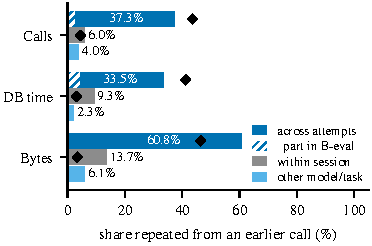
\includegraphics[height=1.62in]{figures/fig1a_scope}}\hfill
  \subcaptionbox{Reuse grows with $N$ (potential tier)\label{fig:ncurve}}{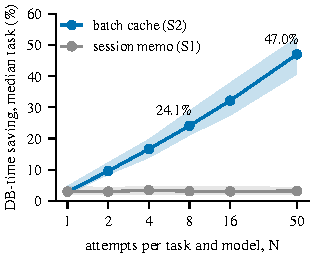
\includegraphics[height=1.62in]{figures/fig1b_ncurve}}\hfill
  \subcaptionbox{What each admission tier admits\label{fig:tiers}}{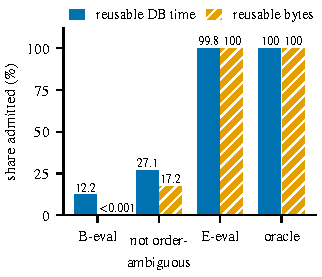
\includegraphics[height=1.62in]{figures/fig1c_tiers}}
  \caption{Where the database work of repeated agent runs repeats, and how much of it each admission tier can reuse
  on DAB. (a) Shares of calls, isolated DB-execution time and payload
  bytes among the 70,173 oracle-admitted calls, by the scope of the earlier exact repeat. The scopes are another
  attempt of the same task and model, the same session, and another model's or task's runs. Shares are pooled over 200
  random attempt orders. Diamonds mark the median task, and hatching marks the part in the B-eval subset. (b)
  Median-task saving of isolated DB-execution time in an unbounded, oracle-gated simulation with 200 resamples. S1 is
  a per-session cache, and S2 is a cache shared by a batch of $N$ attempts of one model on one task. Bands show the
  task-bootstrap 95\% CI, and $N=50$ uses the 268 of 270 task--model cells with 50 runs. (c) Share of the
  cross-attempt reusable DB time and bytes in the B-eval (certified), E-eval (assumption-based) and oracle (potential)
  subsets. The bar ``not order-ambiguous'' covers all calls except the successful ones with at least two distinct rows
  and no top-level \texttt{ORDER BY}. It is a conservative upper bound for any rule that guarantees serialized bytes across query plans in engine row order.}
  \label{fig:teaser}
  \Description{Three panels. Left: horizontal bars showing that repeats across attempts carry 37.3, 33.5 and 60.8 percent of calls, DB time and bytes, against 6.0, 9.3 and 13.7 percent within a session. Middle: lines showing the batch cache saving rising from 3 to 47 percent of DB time as attempts grow from 1 to 50 while the session cache stays near 3 percent. Right: bars showing the B-eval subset holds 12.2 percent of reusable DB time and almost no bytes, the calls that are not order-ambiguous 27.1 percent of the time and 17.2 percent of the bytes, while the E-eval subset and the oracle admit nearly all.}
\end{figure*}


LLM data agents are rarely run once on a task. A deployment retries a failed attempt or samples several attempts and
keeps the most consistent answer \cite{wang2023selfconsistency,brown2024monkeys}. It also evaluates an agent with $k$
trials per task and serves many users who ask the same question of the same data. Every attempt queries the same
database snapshot again. A cache inside one agent session cannot see that another attempt already ran the same query.
A data agent answers an analytical question by letting an LLM plan and issue database queries through a tool. It then
reads the results and post-processes them in Python \cite{ma2026dab,yao2023react}. The DAB benchmark runs each of its
54 multi-database tasks about 50 times with each of five LLMs against one dataset snapshot \cite{ma2026dab}. One DAB
run issues 5.7 database calls on average, and the 13,482 released runs issue 76,213.

For a data system, this repetition is both an opportunity and a cost. The database time of an attempt is
heavy-tailed. The median attempt spends 28.5\,ms executing its successfully replayed calls in isolation, and the
95th-percentile attempt spends 14.4\,s. A single result reaches 771\,MB when written to a file for the agent's Python
code. Recent work frames agents as a first-class data-system workload. The CIDR'26 vision of agent-first data systems
argues that agents speculate redundantly across attempts \cite{liu2026overlords}. TVCACHE caches tool results across
the parallel rollouts of LLM post-training \cite{kumar2026tvcache}. Reuse for the database calls of agent runs that
span several models and engines raises three open questions. Figure~\ref{fig:teaser} previews the results that answer them.

\begin{itemize}
  \item \textbf{Q1: Locality.} Where does the work repeat: within a session, across attempts of a task, or across
  models and tasks? The answer weights repeats by execution cost and result bytes, not only by call count.
  \item \textbf{Q2: Admissibility.} What can be reused while the agent sees byte-identical results? An exact reuse
  reproduces what a completed call shows the agent: the tool message, the bound value and any result file.
  \item \textbf{Q3: Ownership.} Who owns a reused result? At the tool boundary a result has two consumers. The LLM reads a preview, and the agent's Python code reads a file. Its owner decides what it costs to store and whether
  one attempt can corrupt it for another.
\end{itemize}

We answer these questions with a replay-based study of the public DAB release. We re-execute the 41,616 distinct
database--query pairs of the 13,482 runs in isolation, up to three times each, in a version-pinned runtime. The replay
uses the benchmark's own execution and serialization path. It attaches an execution cost, a result size and a
fidelity record to every replayed call. We attribute each call to the innermost scope in which an exact-text
equivalent occurred earlier. We resample $N$ attempts per task and model to measure how reuse grows with $N$. We
separate three admission tiers: what a static certificate admits, what a pinned runtime reproduces, and what an oracle
could reuse. We then compare six reuse designs at the tool boundary with an exact-accounting simulator and with live
runs. The live runs return the harness's exact tool messages and files and execute the agents' own Python consumers.

\textbf{F1: Cross-attempt locality.} We consider the calls whose replay is equivalent to the recorded observation. Exact repeats from other attempts of the same task and model carry 33.5\% of the isolated DB-execution time and 60.8\% of the result bytes. Repeats within the same session carry 9.3\% and 13.7\%. Per task the contrast is sharper, with medians of
41.2\% against 3.2\% and a larger cross-attempt median in all 12 datasets. In an unbounded simulation, a cache shared by a batch saves 24.1\% of the median task's oracle-admitted DB time at eight attempts. It
saves 47.0\% at fifty attempts, while a per-session cache stays near 3\% at every $N$. Four public leaderboard
harnesses that run DAB's tasks with other agent designs show the same ordering.

\textbf{F2: Certifiability--payoff divergence.} The cross-attempt payoff is recovered by runtime qualification rather
than by static certification. A conservative static certificate of byte stability admits 7.5\% of all calls and
0.023\% of the payload bytes. Of the cross-attempt reusable work it admits 12.2\% of the DB time and 0.00005\% of the
bytes. No sharper rule with the same across-plan guarantee closes the gap. The reason is that 58.7\% of the successful calls return at least two distinct rows without a top-level \texttt{ORDER BY}. A pinned runtime that we qualified offline
recovers the payoff in this workload. Every statically admissible DAB call whose replay succeeded was byte-stable. So
was every statically admissible query from four additional harnesses whose replay succeeded. Byte stability of these
calls is thus an empirical property of the qualified runtime.

\textbf{F3: Ownership governs storage cost.} This exploratory study uses the calls that the offline-qualified pinned runtime reproduces. At eight attempts, a simulated private-copy cache writes 1.70$\times$ the no-sharing bytes for the median task. A read-only shared
store with one alias per attempt writes 0.448$\times$ the bytes of private copies for the median task with spilled
results. It keeps 0.76$\times$ the peak footprint of no sharing when every attempt's outputs are retained. On the 12
calibration cells, live bytes written and footprint match the simulator in all 480 runs. The shared store reaches the
footprint of copy-on-write clones without reflink support and refuses the agents' writes. A live tool-boundary replay
covers one eight-attempt batch from each of the 270 task--model cells, 11,309 calls in all. Among its 2,443 cached hits, no cached value differed where both designs returned a result. Two hits returned a result where the uncached execution failed under load. All 4,655 consumer executions whose two uncached runs agreed produced the same output under reuse. Reference pinning keeps aliases valid under concurrent attempts.

This paper makes four contributions. The first is a replay-based methodology for the database work of repeated agent runs (Section~\ref{sec:method}). It yields a cost and fidelity table for 41,616 distinct agent queries and three admission tiers. The second is a characterization of where that work repeats and how reuse grows with the
number of attempts (Section~\ref{sec:locality}). The third is a measurement of how much reusable work each admission
tier admits (Section~\ref{sec:certify}). The fourth is a case study of result ownership at the tool boundary
(Section~\ref{sec:ownership}). Section~\ref{sec:boundaries} delimits the scope and derives design implications.

\section{Preliminaries}
\label{sec:background}



\paragraph{Tool boundary.}
DAB gives an agent a natural-language question over one or more databases of a dataset and a tool interface. The agent
runs a reason-and-act loop \cite{yao2023react} until it returns an answer \cite{ma2026dab}. The \texttt{query\_db}
tool executes an SQL query on SQLite, DuckDB or PostgreSQL, or a find specification on MongoDB. It serializes the
result as JSON and stores it under a key that the agent's later Python code can read. A result of at most 10,000
characters is returned to the LLM in full and bound to the key as a value. A longer result is written to a JSON file
in the attempt's working directory, and the key is bound to the file path. The LLM then sees only the first 10,000
characters as a preview. The \texttt{execute\_python} tool runs agent-written code against these bindings. A result
thus has two consumers: the LLM reads the preview, and the agent's code reads the file. Of the successfully replayed
calls, 25.9\% produce such a spilled file.

\paragraph{Attempts and batches.}
We call one run of one model on one task an \emph{attempt}, and the state an attempt accumulates its \emph{session}.
Repeated attempts arise from retries, from sampling several attempts per question
\cite{wang2023selfconsistency,brown2024monkeys}, from $k$-trial evaluation, and from users who ask the same question.
We study \emph{batches}: $N$ attempts of one model on one task against one static database snapshot.  The data do not change within a batch, so no cached result is ever invalidated.

\paragraph{Result-preserving reuse.}
A reuse design serves a later call with the bytes that an earlier exact-text equivalent call produced, for the same
database and query text. Reuse is \emph{result-preserving} if the later attempt sees exactly what a completed execution
of the call in the same runtime returns. This covers the tool message, the bound value and the content of any file.
The property belongs to the runtime: it holds for a call when re-executing it there returns the same bytes. The
property is conditional on completion. Whether a fresh execution completes also depends on the load, which no
admission rule controls. Where a fresh execution would time out, a hit shows the agent a result instead of a failure,
and Section~\ref{sec:e2e} counts these cases. Exact text is a conservative equivalence, and Section~\ref{sec:keys}
measures what stronger keys add. The three questions of Section~\ref{sec:intro} thus become concrete. Q1 asks in
which scope an exact repeat occurs. Q2 asks for which calls reuse is result-preserving and how a system can know it.
Q3 asks which component holds the reused bytes: the cache, the attempt or a shared store.

\section{Methodology}
\label{sec:method}



\paragraph{Workload.}
We use the public DAB release \cite{ma2026dab}: 13,482 of its 13,500 runs of five LLMs on 54 tasks over 12 datasets.
The LLMs are Gemini-2.5-Flash, Gemini-3-Pro, GPT-5-mini, GPT-5.2 and Kimi-K2, and the databases run on SQLite,
DuckDB, PostgreSQL and MongoDB. Parsing the trajectories yields 151,293 tool calls, of which 76,213 are
\texttt{query\_db} calls. Re-running each task's own validator on the final answers gives 4,543 passing and 8,939
failing runs. Table~\ref{tab:datasets} lists the datasets, which range from 0.6\,MB to 5.6\,GB on disk. The traces
record what each call returned but not what it cost, so we measure cost by replay.

% Table -- the 12 datasets (full width, Section 3)
\begin{table*}[tbp]
  \caption{The 12 DAB datasets of the workload. Columns give the engines (S: SQLite, D: DuckDB, P: PostgreSQL, M:
  MongoDB), the tasks, and the size on disk of the database files and dumps as shipped. They also give the
  \texttt{query\_db} calls, the distinct (database, query) pairs, and the share of successfully replayed calls whose
  result spills to a file. Isolated DB-execution time and payload bytes are summed over all calls. The last columns
  give the median over the dataset's tasks of the DB-time share repeated from other attempts and within the session
  (potential tier).}
  \label{tab:datasets}
  \small
  \begin{tabular}{@{}llrrrrrrrrr@{}}
\toprule
 & & & Data & & Distinct & Spilled & DB time & Bytes & \multicolumn{2}{c}{Task-median repeat \%} \\ \cmidrule(l){10-11}
Dataset & Engines & Tasks & (MB) & Calls & pairs & \% & (s) & (GB) & other attempts & session \\
\midrule
agnews & S, M & 4 & 40.6 & 4,240 & 1,360 & 32.8 & 196 & 11.07 & 41.8 & 2.3 \\
bookreview & S, P & 3 & 1.7 & 3,060 & 1,093 & 49.6 & 5 & 0.11 & 51.8 & 4.3 \\
crmarenapro & S, D, P & 13 & 32.8 & 16,879 & 10,412 & 11.7 & 73 & 0.39 & 35.5 & 1.8 \\
DEPS\_DEV\_V1 & S, D & 2 & 549.9 & 3,125 & 1,281 & 57.1 & 1,874 & 76.06 & 22.3 & 6.9 \\
GITHUB\_REPOS & S, D & 4 & 928.5 & 6,061 & 3,159 & 35.8 & 7,261 & 222.55 & 54.4 & 9.8 \\
googlelocal & S, P & 4 & 0.6 & 3,779 & 1,482 & 16.0 & 5 & 0.03 & 53.9 & 5.0 \\
music\_brainz\_20k & S, D & 3 & 3.1 & 2,451 & 1,071 & 23.2 & 32 & 1.67 & 50.0 & 0.8 \\
PANCANCER\_ATLAS & D, P & 3 & 301.4 & 6,716 & 4,045 & 43.4 & 211 & 1.05 & 37.9 & 3.6 \\
PATENTS & S, P & 3 & 5,556.3 & 4,263 & 2,322 & 63.0 & 23,398 & 225.08 & 36.1 & 7.1 \\
stockindex & S, D & 3 & 4.5 & 2,663 & 1,214 & 25.8 & 64 & 2.70 & 30.7 & 0.6 \\
stockmarket & S, D & 5 & 965.7 & 14,481 & 10,767 & 14.6 & 5,398 & 0.11 & 14.4 & 1.5 \\
yelp & D, M & 7 & 3.7 & 8,495 & 3,410 & 17.2 & 36 & 0.14 & 52.4 & 7.9 \\
\midrule
All &  & 54 & 8,388.9 & 76,213 & 41,616 & 25.9 & 38,553 & 540.96 & 41.2 & 3.2 \\
\bottomrule
\end{tabular}

\end{table*}

% Table -- workload, replay coverage and fidelity by engine (column width, Section 3)
\begin{table}[htbp]
  \caption{Replay coverage and fidelity by engine. Columns give the distinct (database, query) pairs and the share of calls
  whose replay succeeded. They also give the share of successful calls whose replayed result is byte-identical to
  the recorded observation. Byte mismatches differ only in row order or otherwise, and load-time object identifiers
  explain 1,299 of the 1,757 MongoDB mismatches. For spilled results, fidelity compares the 10,000-character preview that the trace keeps.
  The six pairs whose database is not in the task's configuration were not replayed.}
  \label{tab:workload}
  \small\setlength{\tabcolsep}{2.6pt}
  \begin{tabular}{@{}lrrrrrr@{}}
\toprule
 & & Distinct & Replay & Byte- & \multicolumn{2}{c}{Mismatches} \\ \cmidrule(l){6-7}
Engine & Calls & pairs & ok \% & identical \% & order & other \\
\midrule
DuckDB & 29,145 & 18,569 & 94.0 & 91.7 & 1,743 & 520 \\
MongoDB & 8,508 & 3,292 & 96.4 & 78.5 & 0 & 1,757 \\
PostgreSQL & 19,033 & 11,712 & 88.4 & 94.3 & 547 & 406 \\
SQLite & 19,455 & 8,037 & 98.5 & 99.9 & 0 & 4 \\
\midrule
All & 76,213 & 41,616 & 93.9 & 93.0 & 2,290 & 2,687 \\
\bottomrule
\end{tabular}

\end{table}


\paragraph{Isolated replay and fidelity.}
The 76,213 calls contain 41,616 distinct (database, query) pairs, and 66 calls lack a complete database or query
argument. We execute each pair three times in isolation in a version-pinned runtime through DAB's own execution and
serialization code. The runtime is a container image with Python 3.12, DuckDB 1.3.1 restricted to one thread and
pandas 2.3.0. It also holds PostgreSQL 16.15 without parallel workers and MongoDB 7.0.43, and it applies a 120\,s cap.
A pair is not executed again after an execution that reaches the cap. Six pairs name a database that is not in the
task's configuration and cannot be replayed. Hence 41,610 pairs covering 76,141 calls have a replay outcome
(Table~\ref{tab:workload}). Each pair yields an isolated execution time, which is the median of the completed runs.
It also yields serialization and spill times, the size of the serialized result, and a byte-stability flag over the
three results. In all, 37,675 pairs are stable, 3,917 fail, 15 time out and 3 return different values. We compare
each replayed result with the observation recorded in the original run. That observation is the full result when it
was inline and its 10,000-character preview when it was spilled. A replay is byte-identical to it, or equivalent
after normalization. Normalization covers row order, missing-value rendering, float digits beyond the ninth decimal
and MongoDB object identifiers assigned at load time. The two checks answer different questions. Stability over the
three replays is our empirical evidence that reuse is result-preserving inside the pinned runtime. The comparison
with the original run establishes \emph{fidelity}: the replayed cost and size describe the call the agent made. For a
spilled result it covers the preview, because the traces do not keep the file.

\paragraph{Cost model.}
We report two time metrics. \emph{Isolated DB-execution time} is the replayed execution time of a call and measures
the database work that reuse can avoid. \emph{Tool time} is what a design spends per call at the tool boundary. It
covers execution and serialization on a miss, the spill-file write, a cache lookup, and the per-file work on a hit.
The simulator charges the per-operation costs of the first live calibration. A lookup takes 1.27\,\textmu s, an alias
12.6\,\textmu s and a copy 0.46\,ns per byte. A clone, measured in the copy-on-write calibration, takes 0.29\,ms. Two
later calibrations measured the first three costs again and differ from these values by at most 7.3\%. When we
validate the simulator against a live run, it charges that run's costs. A simulation contains the calls that its tier
admits, and savings are relative to executing those calls without reuse. A task's saving is the ratio of its costs
summed over its models and resamples, and we report the median over tasks.

\paragraph{Admission tiers.}
A cache needs an admission rule that decides, before it reuses a result, that reuse is result-preserving. We evaluate
three tiers of decreasing strength (Table~\ref{tab:tiers}). \emph{Certified (Contract B)} is a default-deny whitelist
over the query text and the audited schema, a conditional certificate. Table~\ref{tab:contractb} summarizes its
construct whitelist, and the artifact holds the executable rule with its additional fail-closed checks. The rule
admits one \texttt{SELECT} block over base tables in which every name binds to a stored column. It admits three shapes. The first is one row of counts and extrema. The second is stored columns under an \texttt{ORDER BY} that names every output. The third is groups ordered on their grouping columns. \texttt{SUM}, \texttt{AVG} and the variance family are not on the list, because
their floating-point value depends on the order of accumulation
\cite{mueller2018reproducible,duckdb2026nondeterminism}. Clock-dependent values are excluded as well. On MongoDB,
whose DAB interface has no sort, the rule admits only a lookup by object identifier. The rule certifies byte
stability under three preconditions. P1 requires a fixed snapshot, engine version and session configuration, and a
fresh read-only session. P1 also requires a catalog without objects that act behind the query text, such as
row-level security or user-defined functions. P2 concerns every stored column that the query outputs, groups by or
passes to \texttt{MIN} or \texttt{MAX}. In such a column, values that the engine compares as equal print the same
bytes. P3 requires a deterministic serializer. Under P1--P3, two completing executions of an admitted query return
the same bytes whatever the plan, parallelism or physical row order. The joined and filtered rows form a multiset
that the text and the data determine, and \texttt{COUNT} is a function of that multiset. \texttt{MIN}, \texttt{MAX}
and the grouping range over columns for which P2 holds. The \texttt{ORDER BY} leaves ties only between rows that
print the same. The plan does not decide whether the query raises an error either. Every operation that
Table~\ref{tab:contractb} admits in a row expression returns a value or \texttt{NULL} for every input in the pinned
engines. A one-row output is evaluated exactly once. Contract B thus certifies the bytes of an execution that
completes. Whether a fresh execution completes within its resource limits depends on the query, the data, the limits
and the load. Completion therefore lies outside the certificate. P2 is a property of the data that the query text
cannot establish. A column that holds both $0.0$ and $-0.0$, or both $1$ and $1.0$, violates it. We therefore audit
the snapshot: all 19,772 stored columns of DAB's 26 SQL databases satisfy P2, and their catalogs hold no such object.
A unit suite of 181 assertions tests the implementation. Section~\ref{sec:threats} reports how the rule evolved after
the experiment plan and how its argument was checked.

\emph{Assumption-based (Contract E)} keeps the read-only, determinism and allow-list checks and drops the ordering
and shape checks. Byte stability then also rests on the runtime reproducing the engine's physical row order. Without a sort, the engines leave that order unspecified \cite{postgres2026order,sqlite2026select,mongodb2026sort}. We pin it through the engine version, one thread and a static snapshot. \emph{Potential (oracle)} is the population on
which we measure repeated work rather than an admission rule. It contains every call whose replay is equivalent to
its recorded observation, so that the replayed cost and size describe the call the agent made. It bounds what an
exact cache could reuse and cannot be computed before execution. Counting only byte-identical replays leaves the scope shares almost unchanged (Section~\ref{sec:robust}). Both static rules
are decided before execution. To measure designs, we restrict each rule to the calls whose replay succeeded, is
byte-identical to the recorded observation and is stable over three runs. These are the \emph{B-eval} and
\emph{E-eval subsets}. They are post-hoc evaluation restrictions that apply the same gates to both rules, so the two
subsets differ only in the rule.

% Table -- admission tiers (column width, Section 3)
\begin{table}[htbp]
  \caption{Admission tiers and the calls each admits (of 76,213). ``Online'' means decidable before the call executes.
  The B-eval and E-eval subsets keep the calls of each static rule whose replay was byte-identical to the recorded
  observation and stable over three replays. They are post-hoc restrictions on which we measure designs.}
  \label{tab:tiers}
  \small\setlength{\tabcolsep}{3pt}
  \begin{tabular}{@{}L{1.55cm}L{3.75cm}cr@{}}
\toprule
Tier & Admission rule & Online & Calls \\
\midrule
Certified & Contract B: conditional static byte-stability certificate & yes & 5,697 \\
 & \quad B-eval subset (post hoc) & no & 5,695 \\
Assumption-based & static Contract E, byte stability from a pinned runtime & yes & 74,894 \\
 & \quad E-eval subset (post hoc) & no & 66,263 \\
Potential & oracle: replay equivalent to the recorded observation & no & 70,173 \\
\bottomrule
\end{tabular}

\end{table}

% Table -- Contract B in full (column width, Section 3)
\begin{table}[htbp]
  \caption{Summary of Contract B's construct whitelist. Admission also applies the schema-binding, type-family,
  argument-form, alias and potentially-raising-expression checks of the artifact. $c$: a stored column that satisfies P2.}
  \label{tab:contractb}
  \footnotesize\setlength{\tabcolsep}{3pt}
  \begin{tabular}{@{}L{1.25cm}L{6.7cm}@{}}
  \toprule
  Statement & one \texttt{SELECT} block; no \texttt{WITH}, subquery, set operation, window, \texttt{DISTINCT ON},
  \texttt{VALUES} or table function \\
  \texttt{FROM} & base tables of the audited schema, joined by \texttt{JOIN}\,\ldots\,\texttt{ON} or a comma; no
  \texttt{USING}, \texttt{NATURAL} or \texttt{LATERAL} \\
  Names & each column binds to exactly one stored column of the tables in scope (ASCII names, the engine's case
  rule); an output alias does not shadow another column \\
  Row\newline expression & in \texttt{WHERE}, \texttt{ON} and the argument of \texttt{COUNT}: columns; literals without
  clock words; comparisons; \texttt{AND}, \texttt{OR}, \texttt{NOT}; \texttt{IS NULL}; \texttt{IN} over a list;
  \texttt{BETWEEN}; \texttt{LIKE} with a literal pattern; searched \texttt{CASE}; \texttt{COALESCE};
  \texttt{LOWER}, \texttt{UPPER}, \texttt{LENGTH}, \texttt{TRIM}, \texttt{REPLACE}. SQLite also: arithmetic,
  \texttt{ROUND}, \texttt{SUBSTR}, casts. DuckDB also: \texttt{SUBSTR}, \texttt{TRY\_CAST}, and arithmetic,
  \texttt{ABS} and \texttt{ROUND} over floating-point columns; a string meets only strings in a comparison \\
  One row & no \texttt{GROUP BY}, \texttt{HAVING}, \texttt{ORDER BY}, \texttt{OFFSET} or \texttt{DISTINCT}; each
  output built from \texttt{COUNT}, \texttt{MIN}($c$), \texttt{MAX}($c$), literals, arithmetic and the functions above \\
  Ordered & no aggregate; each output is a column $c$; \texttt{ORDER BY} names every output \\
  Grouped & \texttt{GROUP BY} columns $c$; each output is a grouping column or one \texttt{COUNT},
  \texttt{MIN}($c$) or \texttt{MAX}($c$); \texttt{HAVING} over such aggregates; \texttt{ORDER BY} names every
  grouping column, or every output \\
  Limits & \texttt{LIMIT} (at least one row) and \texttt{OFFSET} take integer literals; plain \texttt{DISTINCT}
  needs an \texttt{ORDER BY} over every output \\
  \bottomrule
  \end{tabular}
\end{table}


\paragraph{Scope attribution and resampling.}
Within each dataset, we order attempts randomly. We assign every oracle-admitted call the innermost scope in which an
exact-text equivalent occurred earlier. The scopes are the same session, another attempt of the same task and model, and another model on the same task. The outermost scopes are another task of the dataset and none. Shares are means over 200 random orders,
weighted by calls, by isolated DB-execution time and by payload bytes. To measure how reuse grows with the number of
attempts $N$, we sample $N$ attempts per task and model without replacement. We use 200 resamples for $N \in
\{1,2,4,8,16,50\}$. For each such batch we simulate a session cache (S1) and a cache shared by the batch's attempts,
both unbounded and starting empty. We label the latter S2. Without a budget, its DB-execution saving is the same for every cross-attempt design of Section~\ref{sec:designs}. Those designs differ in what they do with the result file. In all,
268 of the 270 task--model cells have the 50 runs that $N=50$ needs. We report medians over the 54 tasks with
task-bootstrap 95\% confidence intervals and check them with a bootstrap that resamples whole datasets. We test
paired differences with Wilcoxon signed-rank tests, Holm-corrected over a family of 29 tests. Hypotheses and success criteria were fixed in an experiment plan after a pilot replay of the SQLite and DuckDB calls. These are 64\% of the calls. The plan preceded the full replay, and Section~\ref{sec:prereg} reports the outcomes.

\paragraph{Instruments.}
A trace-driven simulator replays sampled attempt orders through each design of Section~\ref{sec:designs}. It accounts
the tool time, bytes written and peak footprint of every call. A live runner executes the same designs for real on
the calibration cells. These are 12 task--model cells chosen in advance to span each engine's inline-only, mixed and
spill-heavy tasks. The runner returns DAB's exact tool messages and writes real files. Its bytes written and peak
footprint match the simulator exactly in all 480 runs of the E-eval calibration. A live tool-boundary trace replay
runs the designs on one eight-attempt batch from each of the 270 task--model cells. It re-issues each attempt's
recorded database calls and re-runs its recorded Python consumers at their trace position against each design's
bindings. It also probes the shared store with write and delete attempts, and the LLM is not re-run. A threaded
stress test runs attempts concurrently against one shared store. A clean-room job re-parsed the original archive and
re-ran the scope and saving analyses. It reproduced all 8,546 values in their result files to a relative tolerance of
$10^{-9}$. Four further seeds leave the scope shares unchanged and move the $N=4$ median saving by at most 0.6 points.

\paragraph{Environment.}
Every replay, simulation and live run ran as a batch job in Singularity containers on CPU nodes of a university
cluster. The nodes are two-socket x86-64 machines with 28 or 36 cores and 180\,GiB of memory. Each job received the
cores and memory it requested, without exclusive use of its node. A replay executes each query up to three times in
a row after its dataset is loaded. We report the median of the completed executions, and Section~\ref{sec:robust}
weights by the first one instead. Jobs that share a node can slow a run, and the median of three executions damps
this. The live calibration runs every design of a cell within one job, in a random order per resample.

\section{Locality of Reuse}
\label{sec:locality}

This section answers Q1 on the oracle-admitted calls of the potential tier. For every call whose replay is
equivalent to the recorded observation, it locates the first earlier exact repeat.

\subsection{Cross-Attempt Locality}
\label{sec:scope}

Figure~\ref{fig:scope} decomposes the 70,173 oracle-admitted calls by the innermost scope of an earlier exact repeat.
Repeats from other attempts of the same task and model carry 37.3\% of the calls. They carry 33.5\% of the isolated DB-execution time and 60.8\% of the payload bytes. Repeats within the same session carry 6.0\%, 9.3\% and 13.7\%.
Repeats seen only in another model's or another task's runs add 4.0\%, 2.3\% and 6.1\%. Cross-attempt repeats are
skewed toward large results, since they carry 60.8\% of the bytes and 33.5\% of the time. The files that hold large
results are therefore the main target for a cache (Section~\ref{sec:ownership}).

The per-task picture is sharper than the pooled one. The median task attributes 41.2\% of its DB time to
cross-attempt repeats (95\% CI 36.1--49.3\%) and 3.2\% to repeats within a session (2.2--4.6\%). For bytes the
medians are 46.4\% and 3.5\%. The paired difference is significant over the 54 tasks (Wilcoxon, Holm-corrected
$p=2.6\times10^{-9}$, rank-biserial $r=0.997$). It survives the nesting of tasks in datasets. A bootstrap that
resamples whole datasets gives 41.2\% (34.6--50.2\%) against 3.2\% (1.8--6.5\%). The cross-attempt median exceeds the
session median in all 12 datasets (Table~\ref{tab:datasets}, sign test $p=0.0005$). Task by task
(Figure~\ref{fig:pertask}), the cross-attempt share of DB time exceeds the session share in 53 of the 54 tasks. It is
at least three times as large in 51. For bytes the counts are 52 and 43.

\subsection{Scaling with the Number of Attempts}
\label{sec:growth}

Cross-attempt locality turns into savings that grow with the number of attempts. Figure~\ref{fig:ncurve} shows an
unbounded, oracle-gated simulation. A cache shared by the batch (S2) saves 9.6\%, 16.6\%, 24.1\%, 32.2\% and 47.0\%
of the isolated DB-execution time at $N=2$, 4, 8, 16 and 50. These values are medians over tasks on the
oracle-admitted calls. A session cache (S1) stays between 3.0\% and 3.4\% at every $N$. The median task reaches a
20\% saving at $N=8$, where 64.8\% of tasks reach it. At $N=4$, 35.2\% of tasks already save at least 20\% and
79.6\% at least 10\%. The per-task ratio of S2 to S1 DB time falls from 0.943 at $N=2$ to 0.801 at $N=8$. The Holm-corrected $p$ is $4.6\times10^{-9}$ at $N=2$, 4 and 8. Payload bytes follow the same curve, with 23.9\% saved at
$N=8$. Resampling whole datasets widens the $N=8$ interval to 18.4--30.3\% without moving the median. The saving does
not depend on which of the three replays supplies a query's time. At $N=8$ it is 24.1\% (task-bootstrap 95\% CI
21.1--28.8\%) with the median of the completed executions. It is 23.3\% (20.9--28.1\%) with the first execution and
24.1\% (21.1--28.9\%) with the steady-state ones.

\subsection{Heterogeneity and Robustness}
\label{sec:robust}

% Fig. 2 -- locality per task and under different conditions (figure*, Section 4)
\begin{figure*}[tbp]
  \centering
  \subcaptionbox{Per task: session share against cross-attempt share\label{fig:pertask}}{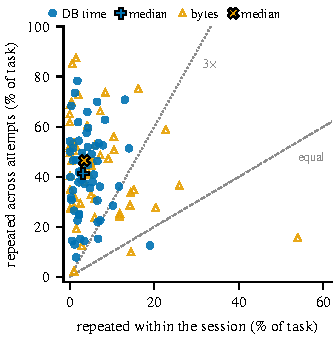
\includegraphics[height=2.05in]{figures/fig2a_pertask}}\hfill
  \subcaptionbox{Pooled share of isolated DB-execution time under different conditions\label{fig:conditions}}{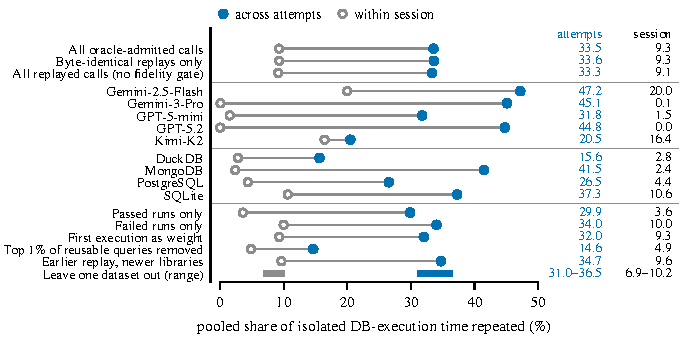
\includegraphics[height=2.05in]{figures/fig2b_conditions}}
  \caption{Locality per task and under different conditions. (a) One point per task and weight for the 54 tasks, on the oracle-admitted calls. Circles show isolated
  DB-execution time and triangles payload bytes. The axes give the share repeated within the session ($x$) and
  across attempts of the same task and model ($y$). The dashed line is $y=x$, the dotted line is
  $y=3x$, and large markers are task medians. (b) Pooled DB-time shares on the 70,173 oracle-admitted calls, a named
  subset, or another population. Byte-identical replays cover 66,556 calls, all replayed calls 76,141, and the earlier
  replay its 62,419 byte-identical calls. Shares are means over 200 random attempt orders, with 20 orders for the two
  gate variants and 50 for the top-1\% removal.}
  \label{fig:locality}
  \Description{Two panels. Left: a scatter plot with two points per task, one for DB time and one for bytes. Nearly all lie above the equal-share line and most above the three-times line. Right: one row per condition. The cross-attempt estimate lies to the right of the within-session estimate in every row, with the leave-one-dataset-out row shown as ranges.}
\end{figure*}


Every model repeats more across attempts than within its session, by different margins
(Figure~\ref{fig:conditions}). GPT-5.2 and Gemini-3-Pro almost never re-issue a query inside a session and repeat
44.8\% and 45.1\% of their DB time across attempts. Gemini-2.5-Flash and Kimi-K2 also repeat inside their sessions
(20.0\% and 16.4\%). At $N=4$ the median task--model saving ranges from 9.0\% for GPT-5-mini to 23.5\% for
Gemini-2.5-Flash.

The ordering persists across engines, fidelity gates, run outcomes, time weights, query removal, dataset removal and
an earlier replay (Figure~\ref{fig:conditions}). Reusable time is concentrated: 67 of the 6,641 reusable queries
(1\%) hold 68.7\% of it. Removing those queries lowers the pooled cross-attempt share to 14.6\%. The per-task medians
barely move (39.3\% against 2.6\%), and the median $N=8$ saving stays at 22.3\%. The earlier replay used newer
library versions (DuckDB 1.5.6, pandas 3.0.6), no pinned time zone and a less strict check of the database load.

The CIDR'26 vision reports that distinct sub-plans are a small fraction of those generated over many attempts
\cite{liu2026overlords}. We reproduce that statistic on DAB's DuckDB-native calls (179 task--model cells, 27,388
calls). The median share of distinct sub-plans per cell is 21.7\% for single operators. It rises to 77.8\% for
sub-plans of six or more operators, while 54.8\% of whole query texts are distinct. For reusing complete results, whole-query repetition across attempts is what a system can exploit.

\subsection{Generalization across Agent Harnesses}
\label{sec:xharness}

% Table 4 -- cross-harness (column width)
\begin{table}[htbp]
  \caption{Exact-call repetition in four public leaderboard harnesses on DAB's tasks and in the first five runs of the
  released DAB traces. The analysis is at trace level, without replay, on the exact database and query text. Qwen3.8
  denotes Qwen3.8-Flash-Next, and DeepSeek-v4.1 denotes DeepSeek-v4.1-flash. Session and other-attempt columns are
  pooled call shares averaged over 50 random attempt orders. $N{=}5$ is the median share of calls that repeat an
  earlier call among five attempts (50 resamples), over the listed number of tasks with five available runs.}
  \label{tab:xharness}
  \footnotesize\setlength{\tabcolsep}{2.5pt}
  \begin{tabular}{@{}lrrrrr@{}}
\toprule
Harness / model & Runs & Calls & \% session & \% other att. & $N{=}5$ \% (tasks) \\
\midrule
Phoenix-CLI / Opus 5 & 270 & 2,937 & 1.7 & 13.4 & 15.5 (54) \\
DAB scaffold / Qwen3.8 & 270 & 3,294 & 0.1 & 15.9 & 17.9 (54) \\
Scout / GLM-5.2 & 249 & 1,490 & 0.3 & 5.7 & 7.8 (37) \\
Stela / DeepSeek-v4.1 & 264 & 3,306 & 0.2 & 5.0 & 4.9 (48) \\
\midrule
DAB / Gemini-2.5-Flash & 269 & 958 & 18.7 & 14.7 & 30.0 (53) \\
DAB / Gemini-3-Pro & 270 & 1,708 & 0.1 & 23.2 & 24.6 (54) \\
DAB / GPT-5-mini & 270 & 1,388 & 0.5 & 8.6 & 11.2 (54) \\
DAB / GPT-5.2 & 270 & 1,093 & 0.1 & 13.5 & 13.2 (54) \\
DAB / Kimi-K2 & 266 & 2,287 & 11.6 & 8.3 & 13.3 (51) \\
\bottomrule
\end{tabular}

\end{table}


The locality does not stem from DAB's own scaffold. We extracted every database call from the public trace archives
of four leaderboard submissions. They ran DAB's tasks with other agent harnesses and models, up to five trials per
task (Table~\ref{tab:xharness}). In all four, exact repeats across attempts outnumber repeats within a session. The
call shares are 13.4\% against 1.7\% for Phoenix-CLI and 15.9\% against 0.1\% for DAB's scaffold with Qwen3.8. They
are 5.7\% against 0.3\% for Scout and 5.0\% against 0.2\% for Stela. At five attempts the median task repeats
4.9--17.9\% of its calls. We also replay these queries with DAB's tool semantics in the pinned runtime, without a
fidelity comparison with the result the harness recorded. Exact repeats across attempts then account for 6.9\%
against 4.8\% of the replay-stable DB time for Phoenix-CLI. The shares are 12.3\% against 0.0\% for Qwen3.8, 9.4\%
against 0.05\% for Scout and 4.0\% against 0.03\% for Stela. The byte ordering holds for Qwen3.8, Scout and Stela.
For Phoenix-CLI, repeats across attempts and within the session account for 0.2\% and 3.4\% of the replay-stable
bytes. At five attempts, the median-task saving is 13.1\%, 14.4\%, 2.9\% and 2.4\% of the replay-stable DB time.
These medians cover 54, 54, 37 and 48 tasks with five runs that contain database calls. 
The Phoenix-CLI traces carry timestamps, and the median LLM turn between a tool result and the next call takes
5.2\,s. Attempts that run concurrently therefore overlap on their queries, the setting of
Section~\ref{sec:concurrency}.

\section{Certifiability versus Payoff}
\label{sec:certify}

Section~\ref{sec:locality} measured potential under an oracle that knows each recorded observation. A deployed cache
has to decide from the query and the runtime alone, before it reuses anything. This section answers Q2. It
establishes which calls a cache can reuse without changing the observed result, and which of them it can recognize
in advance.

% Table 1 -- funnel (column width)
\begin{table}[htbp]
  \caption{Admission funnel over all 76,213 database calls: pooled shares of calls, isolated DB-execution time (a
  timeout counts at the 120\,s cap) and payload bytes. Gates are cumulative. The last two rows are the post-hoc E-eval
  (assumption-based) and B-eval (certified) subsets. They hold the calls of the static E and B rules whose replay is
  byte-identical to the recorded observation and stable across three replays. The oracle (potential) admits every call
  whose replay is equivalent to the recorded observation.}
  \label{tab:funnel}
  \small\setlength{\tabcolsep}{3pt}
  \begin{tabular}{@{}L{3.15cm}rrrr@{}}
\toprule
Gate (cumulative) & Calls & \% calls & \% DB time & \% bytes \\
\midrule
Successful replay & 71,582 & 93.9 & 94.7 & 100.0 \\
Equivalent to recorded observation (oracle) & 70,173 & 92.1 & 94.2 & 98.8 \\
Byte-identical, stable in 3 replays & 66,556 & 87.3 & 93.9 & 98.8 \\
E-eval subset (static E, post hoc) & 66,263 & 86.9 & 93.6 & 98.7 \\
B-eval subset (static B, post hoc) & 5,695 & 7.5 & 9.4 & 0.023 \\
\bottomrule
\end{tabular}

\end{table}

% Fig. 3 -- admission per engine and the verdicts of the static Contract B rule (column width, Section 5)
\begin{figure}[htbp]
  \centering
  \subcaptionbox{The funnel of Table~\ref{tab:funnel} per engine\label{fig:funnelengine}}{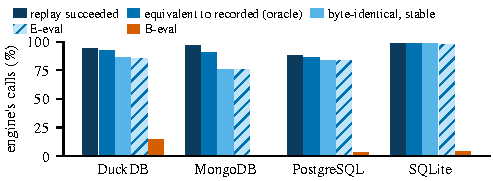
\includegraphics[width=\columnwidth]{figures/fig3a_funnel_engine}}
  \subcaptionbox{Verdicts of the static Contract B rule\label{fig:verdicts}}{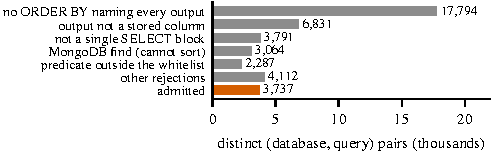
\includegraphics[width=\columnwidth]{figures/fig3b_b_verdicts}}
  \caption{Admission by engine and by rule. (a) Share of each engine's calls that passes each cumulative gate of Table~\ref{tab:funnel}. It covers the 76,141 calls with a replay outcome, and Table~\ref{tab:workload} gives the totals.
  MongoDB's B-eval subset, two calls, is too small to see. (b) Verdict of the static Contract B rule on each of the 41,616 distinct (database, query) pairs. Bars show rejection reasons and the admitted pairs.}
  \label{fig:certify}
  \Description{Two panels. Top: grouped bars per engine showing that most calls of every engine pass the replay, equivalence, byte-identity and E-eval gates, while the B-eval subset is a small share. Bottom: horizontal bars of the number of distinct (database, query) pairs per verdict of the static Contract B rule. The longest bar is the rejection for lacking an ORDER BY that names every output.}
\end{figure}


\subsection{Admission Funnel}
\label{sec:funnel}

Table~\ref{tab:funnel} follows all 76,213 calls through cumulative gates, and Figure~\ref{fig:funnelengine} splits
them by engine. Replay succeeds for 93.9\% of the calls. In all, 92.1\% of the calls reproduce the recorded
observation up to normalization, with 94.2\% of the DB time and 98.8\% of the bytes. A further gate keeps the 87.3\%
that reproduce it byte for byte and stably over three replays. Of the 4,977 byte mismatches between the original
runs and the replay, 2,290 are row-order differences. These comprise 1,743 of 2,263 in DuckDB, which the original
runs used multi-threaded, and 547 of 953 in PostgreSQL. Object identifiers reassigned at load time explain 1,299 of
the 1,757 MongoDB mismatches. After these gates, the static Contract E rule leaves 86.9\% of the calls, the E-eval
subset. Contract B leaves 7.5\%, the B-eval subset.

Before any replay, Contract B admits 5,697 calls (7.5\%) with 9.4\% of the DB time and 0.023\% of the payload bytes.
Every one of these calls completed in each of its replays. For 5,695 of them the original trace records a result,
and every replay is byte-identical to it. This holds although the original runtime ran DuckDB with several threads.
These calls form the B-eval subset, and the remaining 2 have no recorded result. Figure~\ref{fig:verdicts} gives the
rule's verdict on the 41,616 distinct (database, query) pairs. The most frequent rejection, 17,794 pairs, is
\emph{unordered result}: the query is not a one-row aggregate and has no \texttt{ORDER BY} that names every output.
A further 6,831 pairs output something other than stored columns, such as \texttt{SELECT *} or computed values. The
rule accepts 3,507 pairs that return one row of counts and extrema and 228 whose \texttt{ORDER BY} names every
output. It also accepts 2 MongoDB lookups by object identifier.

The gap does not depend on how the rule is written. Of the successful calls, 58.7\% return at least two distinct
rows from a statement without a top-level \texttt{ORDER BY}. They carry 65.0\% of the DB time and 79.2\% of the
bytes of the successful calls. The engines leave the order of such rows unspecified
\cite{postgres2026order,sqlite2026select,mongodb2026sort}, so two correct executions can serialize them differently.
No rule that guarantees the bytes across plans can admit these calls while the tool serializes rows in the order the
engine returns. This holds whatever the rule knows about the schema or the data.

\subsection{Payoff beyond the Certificate}
\label{sec:gap}

Most of the cross-attempt payoff lies outside Contract B. Of the cross-attempt repeats of Section~\ref{sec:scope},
the static B rule admits 6.4\% of the calls, 12.2\% of the DB time and 0.00005\% of the bytes. Its B-eval subset
holds the same shares at this precision. The static E rule admits 99.5\% of the calls and essentially all of the DB
time and bytes. The E-eval subset holds 93.2\% of the calls, 99.8\% of the DB time and essentially all of the bytes
(Figure~\ref{fig:tiers}). Restricting reuse to what Contract B certifies thus forgoes 87.8\% of the reusable DB time
and nearly all of the reusable bytes. A less conservative certificate with the same across-plan guarantee cannot
close the gap. We exclude the successful calls that return at least two distinct rows without a top-level
\texttt{ORDER BY}. The remaining calls are a conservative upper bound for such a rule. They carry 27.1\% of the
reusable DB time and 17.2\% of the reusable bytes. Within each tier's own calls, S2 saves 6.4\% of the median task's
DB-execution time on the B-eval subset (certified) at $N=8$ with an unbounded budget. It saves 24.5\% on the E-eval
subset (assumption-based) and 24.1\% under the oracle (potential).

\subsection{Runtime Qualification}
\label{sec:pinning}

Of the 71,582 calls whose replay succeeded, static Contract E admits 71,275, which cover 37,542 distinct queries.
Inside the pinned runtime every one of them replayed byte-identically three times. Against the observation recorded
in the original runtime, 7.0\% of them differ. These calls carry 0.8\% of their DB time and 1.2\% of their bytes,
and 8.3\% of the repeated calls a cache would serve. Row order alone accounts for 3.2 points and different values
for 2.2. Spilled results whose recorded preview differs account for 1.5, and calls with an error or no result in the
original trace for 0.07. After normalization, 5.1 of the 7.0 points are equivalent. By engine, DuckDB contributes 3.2
points, MongoDB 2.5, PostgreSQL 1.4 and SQLite 0.02. For the calls that Contract E admits and Contract B does not
certify, byte stability is thus an empirical property of the qualified pinned runtime. One pinned runtime reproduced
every admitted result it executed, while two runtimes disagreed on 7.0\% of them. The E-eval numbers are therefore
the payoff under a pinned runtime that was qualified offline. Qualification replays every query three times and
compares it with the recorded observation. The post-hoc gates do not produce that payoff. A cache can apply the
static E rule online and admit every successful call of that rule. S2 then saves 23.8\% of the median task's
DB-execution time at $N=8$, against 24.5\% on the E-eval subset. S3 writes 0.45$\times$ the bytes of S2 in both
cases. The rule also holds on queries it was not written against. The four leaderboard harnesses of
Section~\ref{sec:xharness} issued 8,811 distinct queries whose replay succeeded, 8,382 of them in no DAB trajectory.
Static E, in a code snapshot taken before they were replayed, admits 8,592 of them. Every admitted query returned
the same bytes in three replays. All 27 calls whose replays differed belong to queries that the rule rejects.

\subsection{Reuse-Key Sensitivity}
\label{sec:keys}

Exact text is a conservative key. On the E-eval subset, normalizing whitespace and comments raises the median S2 DB-execution saving from 16.6\% to 17.5\% at $N=4$. At $N=8$ it raises the saving from 24.5\% to 25.2\%. A canonical abstract syntax
tree adds 3.6 and 5.2 points (20.1\% and 29.8\%). An oracle that matches equal results reaches 33.7\% and 48.0\%, or
27.0\% and 37.3\% when empty and single-row results are excluded. It needs the result to decide, so it is a bound,
not a cache.

\section{Result Ownership at the Tool Boundary}
\label{sec:ownership}

Section~\ref{sec:certify} established which calls are reusable. Q3 asks where a reused result should live. This
section is a case study on the E-eval subset of the assumption-based tier. It compares designs that admit the same
calls and save the same execution, and that differ only in who holds the bytes.

% Fig. 4 -- ownership (column width, Section 6)
\begin{figure}[htbp]
  \centering
  \subcaptionbox{Tool-boundary result ownership and the lifetime of a shared object\label{fig:designs}}{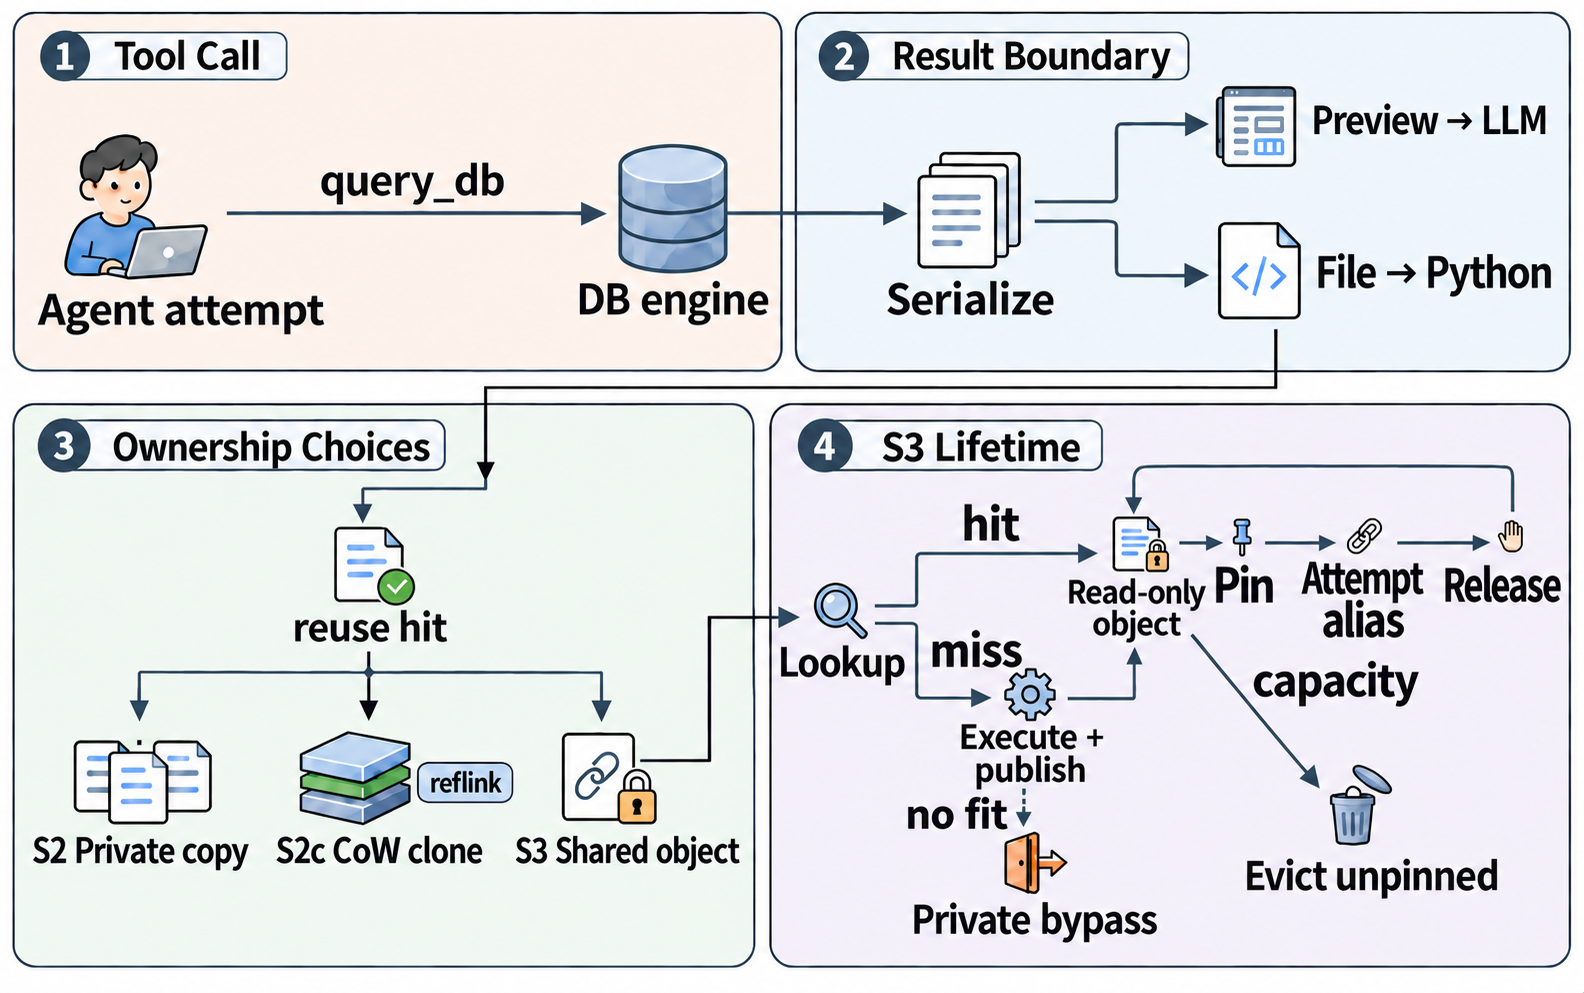
\includegraphics[width=\columnwidth]{figures/fig4a_ownership}}\\[3pt]
  \subcaptionbox{Footprint vs.\ $N$\label{fig:footN}}{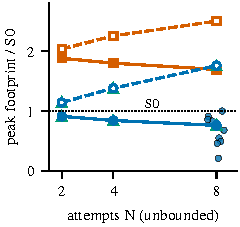
\includegraphics[height=1.45in]{figures/fig4b_footprint_N}}\hfill
  \subcaptionbox{Footprint vs.\ budget\label{fig:footB}}{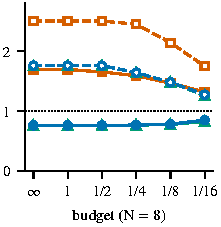
\includegraphics[height=1.45in]{figures/fig4c_footprint_budget}}\\[1pt]
  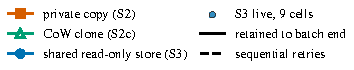
\includegraphics{figures/fig4_legend}
  \caption{Result ownership decides storage cost. (a) A \texttt{query\_db} result is serialized into an LLM preview and a file for Python. Only the file takes part in ownership. On a hit, S2 provides a private copy and S2c a reflink clone. S3 aliases one shared read-only object. SD is omitted because it changes execution but retains attempt-private serialization and files. Section~\ref{sec:designs} describes the lifetime of an S3 object. (b, c) Simulated peak footprint relative to no sharing (S0) on the assumption-based E-eval subset. Values are medians over the 52 tasks with nonzero S0 footprint (50 resamples). Panel (b) uses an unbounded budget and panel (c) uses $N=8$.
  Solid lines retain outputs to batch end, and dashed lines are sequential retries. Dots in (b) are live S3/S0 on the
  9 calibration cells with admitted spilled bytes ($N=8$, unbounded budget, median of 5 resamples, jittered). The
  simulator reproduces each cell.}
  \label{fig:ownership}
  \Description{Top: a four-region diagram. Region 1 shows an agent attempt calling query_db on a database engine. Region 2 shows the result serialized into a preview for the LLM and a file for Python. Region 3 shows three ownership choices on a reuse hit: a private copy, a copy-on-write clone, and a shared object. Region 4 shows the lifetime of a shared object: lookup, hit or miss with execute and publish, pin, attempt alias, release, eviction of unpinned objects under capacity pressure, and a private bypass when a result does not fit. Bottom: two line plots of peak footprint relative to no sharing. Private copies stay above 1, the shared store and clones stay near 0.76 to 0.91 when outputs are retained and between 1.14 and 1.76 for sequential retries.}
\end{figure}


\subsection{Design Space}
\label{sec:designs}

All six designs keep the format of DAB's tool messages and bindings (Figure~\ref{fig:designs}). \emph{S0 Isolated}
executes every call. \emph{S1 Session memo} reuses results within an attempt. \emph{SD} is an execution-only cache
model that caches results inside the engine, as warehouse result caches do
\cite{snowflake2026persisted,google2026bqcache,databricks2026querycache}. A hit skips execution, and every attempt
still serializes the result and writes and keeps its own file. \emph{S2 Private copy} keeps one cached copy of each
result per batch and gives every attempt that hits a private copy of the file. \emph{S2c CoW clone} does the same
with copy-on-write clones that share extents through reflink \cite{rodeh2013btrfs}. \emph{S3 Shared read-only store}
keeps one read-only file per result in a store shared by the batch. It binds an attempt-local alias, a symbolic link,
to that file. 

\paragraph{Shared-store protocol.}
A \emph{lookup} under the store's lock finds the key and moves it to the most-recently-used end. It increments the
key's reference count once per attempt and binds the alias or the inline value. On a \emph{miss}, the attempt
executes and serializes the query. To \emph{publish}, it makes room by evicting least-recently-used objects whose
reference count is zero. It then makes the file read-only and inserts it. If nothing evictable frees enough space,
the result \emph{bypasses} the store and is written as a private file. The attempt's references are \emph{released}
when the attempt ends under the sequential lifetime, or when the batch ends under the retained lifetime. Under
concurrency, a miss follows one of two policies. It executes optimistically and re-checks the table before
publishing, discarding its own copy if another attempt published first. Alternatively it waits for the attempt
already executing that key (\emph{single-flight}).

\paragraph{Design rationale.}
Aliases instead of copies avoid writing a result once per hit. Clones avoid the write too but need a file system with reflink \cite{mkfsxfs2026}. The node-local XFS file systems of our cluster offer reflink, and its GPFS scratch file system does not. Read-only objects keep one attempt's code from accidentally altering a result another attempt reads. Private copies remain writable by design. Pinning keeps eviction from deleting an object behind a
live alias (Section~\ref{sec:concurrency}). Footprint depends on how long outputs live, so we report two lifetimes.
Under the \emph{retained} lifetime, every attempt's outputs stay readable until the batch ends, and S3 holds its
references until then. Under the \emph{sequential} lifetime, attempt-private files are deleted and S3 references
dropped when an attempt ends. Budgets are fractions of a task's distinct admitted stored bytes over all of its runs.
This base depends neither on $N$ nor on the sampled batch. Its median over tasks is 17.4\,MB and its 95th percentile
13.7\,GB.

% Table 2 -- designs (full width)
\begin{table*}[tbp]
  \caption{Reuse designs at $N=8$ with an unbounded budget on the assumption-based E-eval subset (simulation, 50
  resamples). DB-execution saving relative to S0 is the median over 54 tasks. Bytes written and peak footprint
  relative to S0 are medians over the 52 tasks with nonzero S0 writes, under the retained and sequential lifetimes of
  Section~\ref{sec:designs}. Both are exact accounting. Modeled tool-time saving is the simulator's estimate (median
  over 54 tasks), with a per-run error of 43.9\% on this subset. The live calibration
  compares S2, S2c and S3, and SD's tool time is modeled only. Measured primitives are the live copy rate per byte
  (258 copies) and the clone (482) and alias (282) times.}
  \label{tab:designs}
  \small
  \begin{tabular}{@{}lrrrrlr@{}}
\toprule
 & DB-time & Written & \multicolumn{2}{c}{Footprint / S0} & Measured & Modeled tool-time \\
\cmidrule(lr){4-5}
Design & saving \% & / S0 & retained & sequential & primitive & saving \% \\
\midrule
Isolated (S0) & 0.0 & 1.00 & 1.00 & 1.00 & --- & 0.0 \\
Session memo (S1) & 3.4 & 0.98 & 0.98 & 0.96 & --- & 3.4 \\
Execution-only cache model (SD) & 24.5 & 1.00 & 1.00 & 1.00 & --- & 11.8 \\
Private copy (S2) & 24.5 & 1.70 & 1.70 & 2.50 & copy 0.46 ns/B & 24.9 \\
CoW clone (S2c) & 24.5 & 0.76 & 0.76 & 1.76 & clone 0.29 ms & 24.8 \\
Shared read-only store (S3) & 24.5 & 0.76 & 0.76 & 1.76 & alias 12.6\,\textmu s & 25.0 \\
\bottomrule
\end{tabular}

\end{table*}


\subsection{Storage and Time Costs}
\label{sec:storage}

Table~\ref{tab:designs} compares the designs at $N=8$ with an unbounded budget. Every cross-attempt design skips the
same executions and saves 24.5\% of the median task's DB-execution time. The designs differ in what happens to the
result file. In the simulator's tool-time model, the three tool-boundary caches (S2, S2c, S3) save 24.8--25.0\% and
the execution-only model 11.8\%. A hit in the engine still pays serialization and the file write, and the live
comparison of tool time follows below. Storage separates the designs, and its accounting is exact. Private copies
write 1.70$\times$ the bytes of no sharing, since every hit writes a copy, while S2c and S3 write 0.76$\times$. Per
task, S3 writes 0.448$\times$ the bytes of S2 at $N=8$ (95\% CI 0.433--0.459 over the 52 tasks with spilled results).
The ratio is 0.489$\times$ at $N=2$ and 0.336$\times$ at $N=50$, at a simulated tool-time ratio of 0.999. Per engine,
S3 writes at most 0.63$\times$ the bytes of S2 at every $N$ and budget.

Figures~\ref{fig:footN} and~\ref{fig:footB} show the footprint. With outputs retained to the batch end, S3 and S2c
store 0.91$\times$ of no sharing at $N=2$ and 0.76$\times$ at $N=8$, while S2 stores 1.70$\times$. The live runs
measure this footprint directly at the unbounded budget, where nothing is evicted and the reference lifetime cannot
matter. On the 9 calibration cells with admitted spilled bytes, S3 stores 0.68$\times$ of S0 (range 0.21--1.00) and
S2 1.55$\times$. These values equal the simulator cell by cell, and on-disk size matches the accounting in all 180 runs. Under the sequential lifetime S2, S2c and S3 store more than no sharing, because cached results
outlive the attempt that produced them. S3 still stores 25--44\% less than S2, and the budget bounds the excess
(1.27$\times$ of S0 at 1/16).

In our copy-on-write accounting, S2c matches S3 in bytes and footprint. The median per-task ratio of S3 to S2c is 1.000 at every $N$ and budget except the tightest retained one (1/16). There it reaches 1.0029 at $N=8$. In tool
time S3 is slightly ahead, at 0.997--0.999 of S2c across $N$ and budgets, because a clone costs more than an alias.
Live on six calibration cells on a reflink-capable file system, the time-weighted tool-time saving is 59.1\% for S2,
56.3\% for S2c and 59.3\% for S3. A clone costs 0.29\,ms per file against 12.2\,\textmu s for an alias. S2c and S3
both write 0.38$\times$ the bytes of S0, as simulated. The physical footprint of clones and the retained footprint
at finite budgets are simulated, not measured live. 

% Table 3 -- correctness (a) and concurrency (b) (full width, stacked)
\begin{table*}[tbp]
  \caption{Observations under reuse on the assumption-based E-eval subset, $N=8$. (a) Live trace replay of S3 against
  S0 on identical attempt orders. The passes cover all 270 task--model cells (one resample, unbounded budget) and a
  one-worker rerun of the 15 PATENTS cells on the same attempt orders. They also cover the 12 calibration cells
  (budgets $\infty$ and 1/4, two resamples) and a CoW pass on 8 of them. ``Hits $\neq$ S0'' counts cached hits whose
  observation differs from S0. ``Value mismatches'' counts hits where S0 and S3 both returned a result and the
  results differ. The 2 differing hits of the all-cell pass are PATENTS calls whose S0 execution failed under load
  while S3 returned a result. ``Consumers'' counts recorded agent Python code re-run with identical successes,
  identical failures, and differing output. The 2 differing consumers in the CoW pass are S0 timeouts at the 120\,s
  cap. (b) The 8 attempts of each calibration cell as concurrent threads against one S3 store (2 resamples, 757 calls
  per configuration), compared with a serial S0 run.}
  \label{tab:e2e}
  \small
  \subcaptionbox{Live trace replay: S3 against S0\label{tab:e2e-a}}{\begin{tabular}{@{}lrrrrrcc@{}}
\toprule
Pass (S3 vs.\ S0) & Cells & Calls & Hits & Hits $\neq$ S0 & Value mismatches & Consumers same ok\,/\,fail\,/\,diff & Probes refused\,/\,total \\
\midrule
All cells, $\infty$ & 270 & 11,309 & 2,443 & 2 & 0 & 3,381\,/\,1,274\,/\,0 & 630\,/\,630 \\
PATENTS rerun, $\infty$ & 15 & 632 & 159 & 0 & 0 & 289\,/\,102\,/\,0 & 45\,/\,45 \\
Calibration, $\infty$, 1/4 & 12 & 1,394 & 310 & 0 & 0 & 742\,/\,76\,/\,0 & 114\,/\,114 \\
Calibration, CoW pass & 8 & 844 & 162 & 0 & 0 & 434\,/\,46\,/\,2 & 72\,/\,72 \\
\bottomrule
\end{tabular}
}\\[4pt]
  \subcaptionbox{Concurrent attempts against one S3 store\label{tab:e2e-b}}{\begin{tabular}{@{}llrrrrr@{}}
\toprule
Budget & Policy & Mismatches & Executions & Duplicates & Wait (s) & Dangling aliases \\
\midrule
$\infty$ & optimistic & 0 & 663 & 107 & 0 & 0 \\
$\infty$ & single-flight & 0 & 556 & 0 & 59 & 0 \\
$\infty$ & optimistic, unpinned & 0 & 664 & 108 & 0 & 0 \\
1/16 & optimistic & 0 & 675 & 103 & 0 & 0 \\
1/16 & single-flight & 0 & 567 & 0 & 86 & 0 \\
1/16 & optimistic, unpinned & 0 & 681 & 106 & 0 & 21 \\
\bottomrule
\end{tabular}
}
\end{table*}


\subsection{Live Trace Replay}
\label{sec:e2e}

Storage savings matter only if reuse is result-preserving in a running system. The live tool-boundary trace replay executes S0, S1, S2 and S3 on identical attempt orders. It uses one eight-attempt batch from each of the 270 task--model cells. It covers 11,309 calls at an unbounded budget. It re-issues every recorded database call through each design
and compares every tool message, inline value, bound path and file content with S0. It also runs each attempt's
recorded Python consumers at their trace position against each design's bindings. S3's store is read-only while they
run (Table~\ref{tab:e2e-a}). The LLM is not re-run, so every attempt follows its recorded trajectory. S3 served
2,443 cached hits. Among the hits where both designs returned a result, no cached value differed from S0's. Two
hits changed what the attempt saw, a case outside result preservation. S0's own live execution failed under load in a PATENTS cell,
and the cache served the result that S0 failed to produce. The other differences are 49 records over 29 distinct
queries across S1, S2 and S3. They are PATENTS calls where one of the two live executions failed while the other
returned a result. Each of these queries completes in isolated replay, with a median of three runs between 8.5 and
80\,s. The pass ran six multi-gigabyte PATENTS cells side by side. In a one-worker rerun of the 15 PATENTS cells on
the same attempt orders, S0 had no live execution failure. S1, S2 and S3 then differed from S0 only on one
non-admitted \texttt{ORDER BY RANDOM()} call, a miss in every design. None of S3's 159 cached hits differed from S0.
The replay thus establishes equivalence at the tool boundary along fixed trajectories. How an agent would continue
after a differing observation is outside it.

All 4,655 consumer executions whose two S0 runs agreed produced the same output and return code under S3 as under
S0. They comprise 3,381 successes and 1,274 identical failures of the agents' own code. We exclude 14 consumers
whose output differed between two S0 runs on the same bindings. All 630 probes that write to an S3 shared object or
delete it were refused and the objects stayed intact. The same probe programs succeed on S2's private copies. The
calibration pass, which adds budget 1/4, shows no database-call mismatch. Neither does the copy-on-write pass, which
adds S2c, and two of its consumer comparisons differ because S0 timed out.

\subsection{Concurrency}
\label{sec:concurrency}

The attempts of a batch can run at the same time. With LLM turns of seconds, as in the Phoenix-CLI traces
(Section~\ref{sec:xharness}), their database calls interleave. The stress test runs the 8 attempts of each
calibration cell as threads against one S3 store. It compares every observation with a serial S0 run
(Table~\ref{tab:e2e-b}), and no configuration produced a mismatch. With optimistic misses, attempts that miss on the
same key execute it in parallel. In all, 107 of 663 executions (16\%) were duplicates, each producing the bytes of
the published object. Single-flight misses wait for the first execution instead. They execute 16\% fewer queries
for 59\,s of total waiting. The negative control shows why pinning is part of the design. With pinning disabled and
a budget of 1/16, eviction removed objects that running attempts still held. It left 21 aliases dangling at attempt
end, and with pinning it left none. Observations at call time still matched, because each file is read when it is
bound. A later read by the agent's code would have failed. An event-driven simulation covers all cells at $N=8$ with
2\,s of LLM time per turn. Optimistic misses duplicate 2.8\%, 8.1\% and 16.7\% of the execution time at 2, 4 and 8
concurrent attempts. Single-flight waiting takes 5.3--26.3\% of tool latency. Eight concurrent attempts finish the
batch in 0.24$\times$ the sequential makespan.

\subsection{Sensitivity Analysis}
\label{sec:sensitivity}

Across the tested policies and budgets, the eviction policy changes little. LRU, FIFO and clairvoyant eviction give
the same S3/S2 bytes written at $N=8$ (0.45 at budget 1, 0.52 at 1/16). Disabling eviction raises it to 0.60 at 1/16,
because objects stuck in the store force 33,525 bypasses instead of 5,822. The S2 DB-execution saving holds at
24.5\% down to a quarter of the budget base and falls to 22.4\% at 1/16. Inline results carry most of the reusable
execution, with a 9.6\% S2 saving from them alone and 3.4\% from spilled ones. Spilled results carry the
serialization and spill time and all of the storage effect. The S3/S2 written ratio is 1.00 when only inline results
are reused and 0.45 when only spilled ones are. The LLM preview belongs in the cache next to the file. Regenerating
it from the cached file costs 82\,ms per hit. It lowers the live tool-time saving of S2 and S3 on six calibration
cells from 59.1\% and 59.3\% to 52.1\% and 52.7\%. Finally, the simulator's bytes and footprint are exact, and its
tool time is accurate where database time matters. On the three heavy calibration tasks the median per-run error is
12.6\%, and simulated S2 savings are within 0.1--1.1 points of live. On the nine cheap tasks, fixed per-call costs dominate and the median error is 51.7\%. Live and at the unbounded budget, S3 saves at least as much tool time as S2 on all 12 calibration tasks.

\section{Scope and Implications}
\label{sec:boundaries}

Sections~\ref{sec:locality}--\ref{sec:ownership} answered the three questions. This section delimits the scope of
those answers and derives design implications.

\subsection{Pre-specified Analyses}
\label{sec:prereg}

% Table -- pre-specified analyses (full width, Section 7)
\begin{table*}[tbp]
  \caption{Pre-specified analyses and thresholds, fixed in the experiment plan after the pilot and before the full
  replay, and outcomes. Contract B evolved after the plan (Section~\ref{sec:threats}). The outcomes that depend on it
  are given for the rule as planned and for the final rule.}
  \label{tab:prereg}
  \small
  \begin{tabular}{@{}L{3.3cm}L{6.1cm}L{6.7cm}@{}}
\toprule
Analysis & Threshold & Outcome \\
\midrule
B0 replay fidelity & replayed result byte-identical to the recorded observation for $\geq$90\% of the successful calls of every engine & met for DuckDB, PostgreSQL and SQLite (91.7\%, 94.3\%, 99.9\%); MongoDB 78.5\%, and 94.4\% equivalent after the normalization of Section~\ref{sec:method} \\
B1 cross-attempt dominance & other attempts $\geq 3\times$ session in time and bytes, pooled and for the median task, on byte-identical replays of the engines that meet B0 & met on that population (three engines): 3.6$\times$ (time), 4.4$\times$ (bytes) pooled; 14.9$\times$, 12.6$\times$ for the median task. On all oracle-admitted calls (Section~\ref{sec:locality}): 3.6$\times$, 4.4$\times$; 13.0$\times$, 13.4$\times$ \\
B2 practical savings & under S2, the median task saves $\geq$20\% of DB time or $\geq$30\% of bytes at $N=4$ & not met at $N=4$ on the oracle-admitted calls with an unbounded budget (16.6\%, 15.9\%); 24.1\% of DB time at $N=8$ \\
B3 ownership & on the calls that Contract B admits, at $N=2$--8: S3 below S2 in median-task bytes written and peak footprint, tool time within 5\%, same direction in every engine & not met on Contract B, which admits a spilled result in only 11 tasks as planned and 8 under the final rule, with a median S3 write saving of 0\% and 0\%; met on E-eval (exploratory, unbounded budget): S3/S2 writes 0.448--0.489, footprint 0.448--0.696 under both lifetimes, tool time 0.998--0.999; in every engine, writes at most 0.63 and tool time at most 1.03 (footprint was not computed per engine) \\
B4 simulator validity and consumer test & on 12 calibration cells at $N=8$ with an unbounded and a 1/4 budget: simulated tool time within 10\%, bytes within 1\%; consumer outputs identical in $\geq$99\% of cases; writes to shared objects refused & bytes and footprint met (max error 0\%); tool time 8.6\% under B as planned (met), 30.6\% under the final B and 43.9\% on E-eval (not met); consumer test, planned on inputs that Contract B admits and run on E-eval inputs, on 238 recorded Python calls: 238 outputs identical under S2 and S3 with the hash seed fixed (233 with random seeds), 36 of 36 write probes refused by a read-only mount (met) \\
B5 heterogeneity & B1 holds in $\geq 10$ of 12 leave-one-dataset-out folds and for every model & on the B1 population, met in 12 of 12 folds (smallest ratio 3.4$\times$ in time, 4.0$\times$ in bytes) and for 3 of 5 models \\
\bottomrule
\end{tabular}

\end{table*}


Six analyses and their thresholds were fixed in the experiment plan, after the pilot and before the full replay
(Table~\ref{tab:prereg}). The other analyses are exploratory. Their outcomes delimit our claims. MongoDB's replays are
byte-identical to the recorded observation for 78.5\% of its successful calls, against a 90\% bar.
Table~\ref{tab:prereg} therefore evaluates B1 and B5 without MongoDB, and every engine is also reported on its own
(Figure~\ref{fig:conditions}). The cross-attempt share exceeds the session share in each of the four engines.
Savings are stated per $N$. The median task crosses the 20\% threshold at $N=8$, and at the pre-specified $N=4$ it
saves 16.6\%. F3 is an exploratory result of the assumption-based tier, because Contract B admits almost no spilled
payload. Of the 54 tasks, 8 have a B-admitted spilled result, with a median S3 write saving relative to S0 of zero.
The tool-time comparison of S2, S2c and S3 uses the live calibration. The tool time of SD and of the budget and
policy variants is a simulator estimate that we report descriptively. Bytes written and footprint are exact
accounting for the configurations the calibration validated. The simulator's per-run tool-time error is 30.6\% under
Contract B and 43.9\% on the E-eval subset, against a threshold of 10\%. It is 39.6\% on E-eval after calibrating
per-call overheads, and it concentrates on cheap tasks. Cross-attempt dominance holds pooled, for the median task and
in every leave-one-dataset-out fold. It reaches 3$\times$ for three of the five models
(Figure~\ref{fig:conditions}).

\subsection{Threats to Validity}
\label{sec:threats}

Contract B evolved after the experiment plan was fixed, and we report three versions. As planned, it was a rule on
the query text alone. That rule also admitted \texttt{SUM}, \texttt{AVG} and the variance family, explicit
collations and MongoDB lookups with further predicates, 8,417 calls in all. A first revision excluded these and admitted 5,344 calls, and adversarial review showed that it still admitted unstable grouped queries. We replaced the rule by the whitelist of Section~\ref{sec:method} and repaired it over six rounds of LLM review. Five rounds found admitted queries whose bytes can
differ, or operations that can fail under one plan only. The sixth found no such query and one more such operation,
which the final rule excludes. Table~\ref{tab:prereg} gives the outcomes that depend on the rule as planned and
under the final rule. One of them changes its verdict, the simulator's tool-time error under B (8.6\% as planned,
30.6\% with the final rule). The certificate is an argument under stated preconditions that review and tests have
probed, not a mechanized proof. An operation that raised on some rows in a way the argument missed would let one
plan fail where another completes. It would not change the bytes of any completing execution. Neither limit weakens
F2. A query that the rule should not admit would only lower the certifiable share. The order-based bound of Section~\ref{sec:funnel} covers every admission rule that guarantees the serialized bytes across query plans in engine row order.

All cost, certifiability and mechanism numbers come from one benchmark family: DAB's static snapshots and its
benchmark-generated attempts, about 50 per task and model. The four leaderboard harnesses add harness and model diversity on the same tasks, not a second workload. Production agents may repeat differently. Locality and
savings are oracle-gated potential, and the designs are measured on post-hoc subsets. E-eval is an offline
qualification of a pinned runtime, not an online admission rule. The 7.0\% cross-runtime disagreement shows what an
unpinned runtime would change. For a spilled result the traces keep only the preview, so fidelity to the original
run covers its first 10,000 characters. Reproduction of the whole file is shown inside the pinned runtime and the
live runs.  The read-only store guards against accidental writes by agent
code. Code that changes file permissions needs a read-only mount or a separate user. The all-cell trace replay uses one batch per cell and follows the recorded trajectories without re-running the LLM. Spilled MongoDB results pass the equivalence gate for 47.2\% of their bytes. 

\subsection{Design Implications}
\label{sec:implications}

For repeated attempts over a shared static snapshot, three design rules follow from the measurements.
\begin{itemize}
  \item \textbf{Batch-scoped reuse.} Reuse should be shared across the attempts of a batch, not only within a
  session. A session memo recovers about 3\% of DB time at any $N$. A cache shared by the batch recovers 24.1\% of
  the oracle-admitted DB time at eight attempts and keeps growing with $N$ (F1).
  \item \textbf{Offline runtime qualification.} An across-plan static byte certificate alone forgoes most of the
  measured payoff. Contract B admits almost none of the reusable bytes. A runtime with pinned engine version,
  parallelism and snapshot reproduced every statically admissible DAB result it executed. The static E check is
  decidable online. Its byte stability is empirical and held for every admitted DAB and additional-harness query
  whose replay succeeded. A certificate that guarantees the tool's serialized bytes across query plans in the row
  order the engine returns cannot cover the order-ambiguous results. Those results carry most of the measured
  payoff (F2).
  \item \textbf{Single read-only ownership with reference pinning.} Each reused result should have one read-only
  owner. Aliases into a read-only store avoid writing a copy per hit, as do copy-on-write clones where the file
  system supports reflink. Read-only objects keep one attempt's code from altering another's input by mistake.
  Reference pinning keeps aliases valid while the store evicts (F3).
\end{itemize}

\section{Related Work}
\label{sec:related}



\paragraph{Agentic data workloads.}
The vision of agent-first data systems names \emph{agentic speculation}: agents issue many, heterogeneous and partly
redundant queries while exploring. It proposes probes, a probe optimizer with multi-query optimization, approximate
answers and partial-result caching, an agent memory store and branching \cite{liu2026overlords}. It supports the
redundancy claim by counting distinct sub-plans over repeated attempts on BIRD \cite{li2023bird}, which
Section~\ref{sec:robust} reproduces on DAB. Our study measures the claim on released multi-model, multi-engine runs
with costs and bytes attached. It also asks which repeats a system could reuse without changing a result. DAB
\cite{ma2026dab} supplies the tasks and trajectories, and Spider~2.0 and BIRD evaluate text-to-SQL more broadly
\cite{lei2025spider2,li2023bird}. Other work measures the end-to-end cost of SQL agents on big-data engines
\cite{eizaguirre2026bigsql} and argues that agentic exploration of relational systems needs moderation
\cite{jivrajani2026sophrosyne}. Further work budgets the observations an agentic text-to-SQL system makes
\cite{peng2026bapsql} and serves agentic workflows as query plans with LLM operators \cite{wadlom2026helium}.
Agentic workloads have also been characterized for LLM serving \cite{chang2026agentic,yuan2026agentic,zhu2026tracelab}.
These works establish agents as a data-system workload and target the cost of individual runs. We isolate what
repeated runs of the same task duplicate.

\paragraph{Tool-result caching for agents.}
TVCACHE, a stateful tool-value cache, caches the values that tools return across the parallel rollouts of LLM
post-training, including SQL generation. A hit requires the agent's whole tool-call history to match an earlier
sequence, because a tool may change the environment \cite{kumar2026tvcache}. ToolCaching caches the responses of LLM
tool-calling services. It decides which requests are cacheable from their semantics and freshness and combines
bandit-based admission with value-driven eviction \cite{zhai2026toolcaching}. Cortex caches the knowledge that LLM
agents fetch from remote sources and serves semantically similar requests from it, validated by a small LLM judge
\cite{ruan2026cortex}. Our study addresses the database side of evaluation and inference runs. There the calls are
read-only against a static snapshot, and a result depends on the query alone. We establish where the repeated work
lies across four engines and which admission rule makes reuse result-preserving. We also establish who should own a
result that reaches the LLM as a preview and the agent's code as a file.

\paragraph{Result reuse in database systems.}
Semantic caching keeps query results at the client and answers later queries from cached regions
\cite{dar1996semantic}. View matching lets the optimizer answer queries from materialized views
\cite{goldstein2001materialized}, and a column store can recycle the intermediates of earlier plans
\cite{ivanova2009recycling}. Cloud warehouses return persisted results for repeated queries over unchanged data
\cite{snowflake2026persisted,google2026bqcache,databricks2026querycache}. LLM-based canonicalization lets an OLAP
cache recognize semantically equal queries \cite{bindschaedler2026semantic}. Nectar caches derived datasets and the
computations that produce them across datacenter jobs \cite{gunda2010nectar}. SQLShare analyzed the reuse in years
of human analytical SQL \cite{jain2016sqlshare}. These mechanisms reuse work inside or beside the engine. This paper
does not propose a new cache or reuse algorithm. It contributes a measurement methodology for repeated agent
attempts and an ownership study for the reuse that happens after the engine. There a result is serialized, spilled
and handed to an agent's sandbox, which is the cost SD leaves on the table (Table~\ref{tab:designs}).

\paragraph{Sharing work among concurrent queries.}
Multi-query optimization shares common subexpressions among queries optimized together \cite{sellis1988mqo}. GraftDB
folds concurrently running analytical queries so that they share partially built operator state
\cite{kimura2026graftdb}. Both need the queries to be in flight at the same time. An agent's calls are separated by
LLM turns, 5.2\,s at the median in the Phoenix-CLI traces (Section~\ref{sec:xharness}). We therefore reuse completed
results across attempts, which complements concurrent sharing within one. When attempts do overlap, a request for a
result that is still being computed is a delayed hit \cite{keren2026delayedhits}. Our single-flight policy makes
such requests wait for the first execution (Section~\ref{sec:concurrency}).

\paragraph{LLM serving caches, agent traces and agent storage.}
Serving systems reuse prompt prefixes and attention key--value state across requests
\cite{zheng2024sglang,kwon2023pagedattention}. That reuse is orthogonal to database execution, serialization and
file ownership. Work on agent state stores trajectories as a data type \cite{zheng2026trajectorydb} and makes
storage a first-class metric of agent evaluation \cite{yu2026footprint}. It also branches, versions or isolates the
databases agents modify \cite{ang2026branchbench,gou2026git4data,zhou2026atcc,zhou2026chronos}. We isolate the database calls of read-only agent runs and the materialization of their results.

\section{Conclusion}
\label{sec:conclusion}

Repeated runs of LLM data agents re-query the same data, and this paper measured what that repetition offers a data
system. On the 76,213 database calls of DAB's public runs, exact repeats live across attempts rather than within a
session. Reuse shared by a batch of attempts therefore grows with their number, while a session cache stays flat.
An offline-qualified pinned runtime reproduced every statically admissible result it executed and thereby recovers
this payoff. A conservative static certificate covers a small part of the reusable DB time, and its dominant
rejection reason by distinct queries is an unordered result. The same order ambiguity bounds every certificate of
byte stability across query plans. At the tool boundary, a read-only shared store writes 0.448$\times$ as many
bytes as private copies for the median task with spilled results. This holds in the unbounded $N=8$ evaluation on
the E-eval subset. In the tested live replays and concurrency tests, read-only pinned aliases preserved the cached
values and kept eviction from invalidating live references. In this repeated-attempt, static-snapshot setting, the
batch of attempts rather than the session is the unit of reuse.


\begin{acks}
We used generative AI tools (Anthropic Claude Code and OpenAI Codex) during the development and preparation of this
work. These tools were used to provide feedback on experimental methodology, assist with the interpretation and
presentation of experimental results, support literature search, and improve the clarity, organization, drafting, and
editing of the manuscript. Generative AI tools were also used to assist with code implementation and debugging. All
AI-assisted code, mathematical reasoning, and derived expressions were independently reviewed, verified, and, where
necessary, revised by the author before being incorporated into the experiments or manuscript.

\end{acks}

\section*{Artifacts}
\label{sec:artifacts}

All code and data behind this paper are in the supplementary archive submitted with it as one zip file. The
directory \texttt{code/} holds the trajectory parser, the Contract B and E certificates with their unit tests, and
the snapshot audit behind precondition P2. It also holds the isolated replay runner, the analysis and simulator, the
live runner with the trace-replay and concurrency tests, the cross-harness extraction and replay, the statistics,
and the job submission tool. The directory \texttt{results/} holds every result file cited in this paper as strict
JSON or CSV, the per-cell live outputs, and a raw bundle. The bundle contains the parsed call and run tables, the
replay cost tables, and a ledger of the states of the cluster jobs. It also contains the
experiment plan with a record of when it was written and a manifest with SHA-256 checksums. The directory
\texttt{paper/} holds the scripts that build the data figures and tables from \texttt{results/}. It also holds a
number ledger that maps each number printed in the paper to its source file and expression, with a checker that
recomputes them. The archive further contains the container build scripts and package lists of the pinned runtime.
Under \texttt{review-stage/} it contains the prompts, responses and reviewed versions of the adversarial reviews of
Contract B. A \texttt{README.md} gives the commands that rebuild the tables and figures from \texttt{results/} and
the results from the public inputs. The inputs are public. They are the DAB repository and trajectory release
\cite{ma2026dab} at revision \texttt{f6b1ad07} and the trace archives attached to DAB leaderboard pull requests \#94,
\#96, \#99 and \#103. Rebuilding the replay cost table took 34 CPU jobs and 24.1 job-hours. The analyses and
simulations rebuild from the tables in the archive, and the live runs need the public inputs.


\balance
\bibliographystyle{ACM-Reference-Format}
\bibliography{references}

\end{document}
\endinput
